\makeatletter
\def\input@path{{../../}}
\makeatother
\documentclass[../../main.tex]{subfiles}

\graphicspath{
	{../../img/}
	{../img/}
	{img/}
}

\begin{document}
	Если $f$~--- непрерывная функция, а поверхность является гладкой, то такой 
	интеграл существует.

	Координаты центра тяжести материальной поверхности $\pi$ с плотностью $\rho =
	 \rho(x,y,z)$ могут быть найдены по формуле: 
	\begin{gather*}x_0 = \frac{\iint \limits_\pi \rho  x ds}{\iint \limits_\pi 
	\rho ds} =
	 \frac{M_{yz}}{m}, \\
	y_0 = \frac{\iint \limits_\pi \rho  y ds}{\iint \limits_\pi \rho ds} =
	 \frac{M_{xz}}{m}, \\
	z_0 = \frac{\iint \limits_\pi \rho  z ds}{\iint \limits_\pi \rho ds} =
	 \frac{M_{xy}}{m}.
	 \end{gather*}
	
	\subsection{Вычисление ПовИ-1}
	Пусть поверхность $\pi$ задана формулой $\pi \ : \ \vec{r} =
	 \vec{r}(u, v) = (x(u,v), \ y(u,v), \ z(u, v)$, где $(u, v) \in D
	  \subset \R^2$, поверхность $\pi$ является гладкой двусторонней
	   поверхностью. Рассмотрим точку $M_k$.
	\[M_k(x_k, y_k, z_k) \leftrightarrow (u_k, v_k)\]
	Разбиение $\pi$ на части $\pi_k$ соответствует разбиению $D$ на $D_k$, при 
	этом
	 если $M_k \in \pi_k$, то $(u_k, v_k) \in D_k$\\
	$\Delta s_k$ \--- площадь $\pi_k$, обозначим площадь $D_k  = \Delta\sigma 
	_k$\\
	\[\sum^{n}_{k=1} \ f(x_k, y_k, z_k)\Delta s_k = \sum^{n}_{k=1} \ f(x(u_k, 
	v_k),
	 y(u_k, v_k), z(u_k, v_k))\Delta s_k \]
	\[\Delta s_k = \iint \limits_{D_k}\sqrt{EG - F^2}dudv = *  \]
	Под корнем непрерывная от $u, v$ функция. Тогда найдется точка $(\tilde{u_k},
	 \tilde{v_k}) \in D_k$ такая, что $* = \sqrt{EG -F^2} \big|_{\tilde{u}_k
	  \tilde{v}_k} \cdot \Delta \sigma_k = (\sqrt{EG _F^2} \big|_{u_kv_k} 
	  +\alpha_k)
   \Delta \sigma_k$, где $\alpha_k \to 0$ при $\delta \to 0$ (Вытекает из 
   равномерной
    непрерывности). И тогда 
	\[ \sum_{k=1}^{n} f(x_k,y_k, z_k) \Delta s_k = \sum_{k=1}^{n} f(x(u_k, v_k),
	 y(u_k, v_k), z(u_k, v_k)) \sqrt{EG - F^2}\big|_{u_k v_k} \Delta \sigma_k
	  +\alpha,\]
	где $\alpha \to 0$. При $\delta \to 0$ получаем:
	\begin{equation}
	\label{lec23-1}
	\iint \limits_{\pi} f(x,y,z)ds = \iint \limits_Df(x(u,v), y(u,v),z(u,v)) 
	\cdot \sqrt{EG - F^2} du dv
	\end{equation}
    В формуле слева находится ПовИ-1, а справа двойной интеграл по плоской 
    области
     $D$.\\
    \begin{rem}
    Величину $ds = \sqrt{EG - F^2} du dv$ можно называть
     дифференциалом поверхности и ее можно заменить другим выражением:
    \[ds = \sqrt{Eg - F^2} = |[\vec r\,'_u}', \vec{r_v]| 
    du dv =
     |\vec{N}| du dv = \sqrt{A^2 + B^2 + C^2} du dv \] 	
    Пусть $\pi$ определена формулой $z= \phi(x,y)$, где $(x,y) \in D$ ($D$ \---
     замкнутая квадрируемая область). Тогда эту поверхность можно 
     параметризовать
      $x=u, y = v, z= \phi(u,v), \ (u, v) \in D$. Имеем вектор 
      $\vec{r} =
       (u, v, \phi(u,v))$. Имеем:
    \[\vec r\,'_u = (1, 0, \phi'_u) \] 
    \[\vec r\,'_v = (0, 1, \phi'_v)\]
	\[E =(\vec r\,'_u)^2 = 1 + (\phi'_u)^2\]
	\[G =(\vec r\,'_v)^2 = 1 + (\phi'_v)^2\]
	\[F = \ <\vec r\,'_u}', \vec{r_v> = \phi'_u \cdot 
	\phi'_v\]
	\[EG - F^2 = 1 + (\phi'_u)^2 + (\phi'_v)^2 \]
	\[\iint \limits_D f(x, y, z)ds = \iint \limits_D f(u,v, \phi(u,v)) \sqrt{1 +
		 (\phi'_u)^2 + (\phi'_v)^2} dudv = \] \[= \iint \limits_D f(x,y, \phi(x,y))
	  \sqrt{1 + (\phi'_x)^2 + (\phi'_y)^2} dudv \]
	\end{rem}
	\begin{exmps}
	\begin{enumerate}
	\item
	\[ \iint \limits_\pi z^2 ds ,\text{ где $pi$ \--- часть конической 
	поверхности} \] 
	\[\pi: \vec{r} = (u\cos v\sin \alpha, u\sin v\sin\alpha, 
	u\cos\alpha) ,
	  \alpha\in (0, \frac{\pi}{2}) \--\text{постоянная}\] 
	\[0 \leq v \leq 2\pi, \qquad 0 < u \leq a \]
	\[r_u' = (\cos v \sin \alpha, \sin v \sin \alpha, \cos \alpha) \]
	\[r'_v = (-u \sin v \sin \alpha, u \cos v \sin \alpha, 0)  \]
	\[E = 1, \quad G = u^2 \sin \alpha^2, \quad F = -u \cos v \sin^2 \alpha \sin 
	v +
	 u \sin v \sin ^2 \alpha \cos v+0 =0\]
	\[EG - F^2 = u^2 \sin^2 \alpha \]
	\begin{gather*}
	\iint \limits_\pi z^2 ds = \iint\limits_{0<u \leq \alpha} u^2 \cos^2 \alpha
	 \ u \sin \alpha du dv = \sin \alpha \cos ^2 \alpha \int \limits_0^\alpha du
	  \int \limits_0 ^{2\pi} u^3 dv = \\ = 2 \pi \sin \alpha \cos ^2 \alpha 
	  \frac{a^4}{4} =
	   \frac{\pi a^4}{2} \sin \alpha \cos^2 \alpha 
	\end{gather*}
	\item 
	\[\iint \limits_\pi x ds, \text{где $\pi$ \-- часть плоскости} \]
	\[2x+y+z-2=0, \text{расположенной в первой октаиде}\]
	\[z = 2 -2x -y\]
	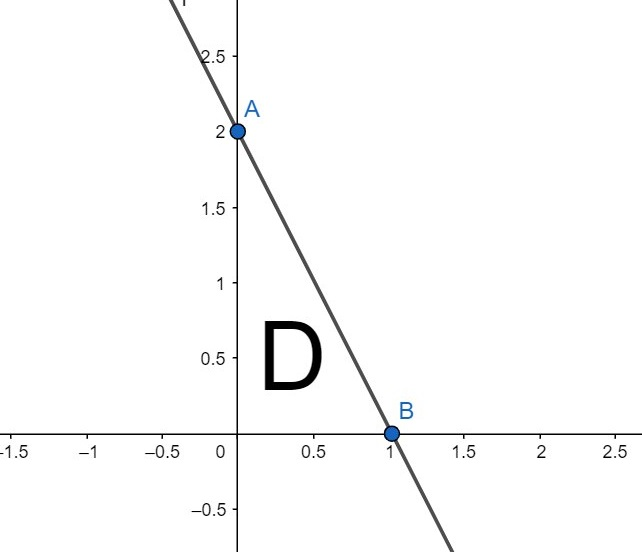
\includegraphics[scale = 0.2]{lec23-1.jpg} 
	\qquad \qquad
		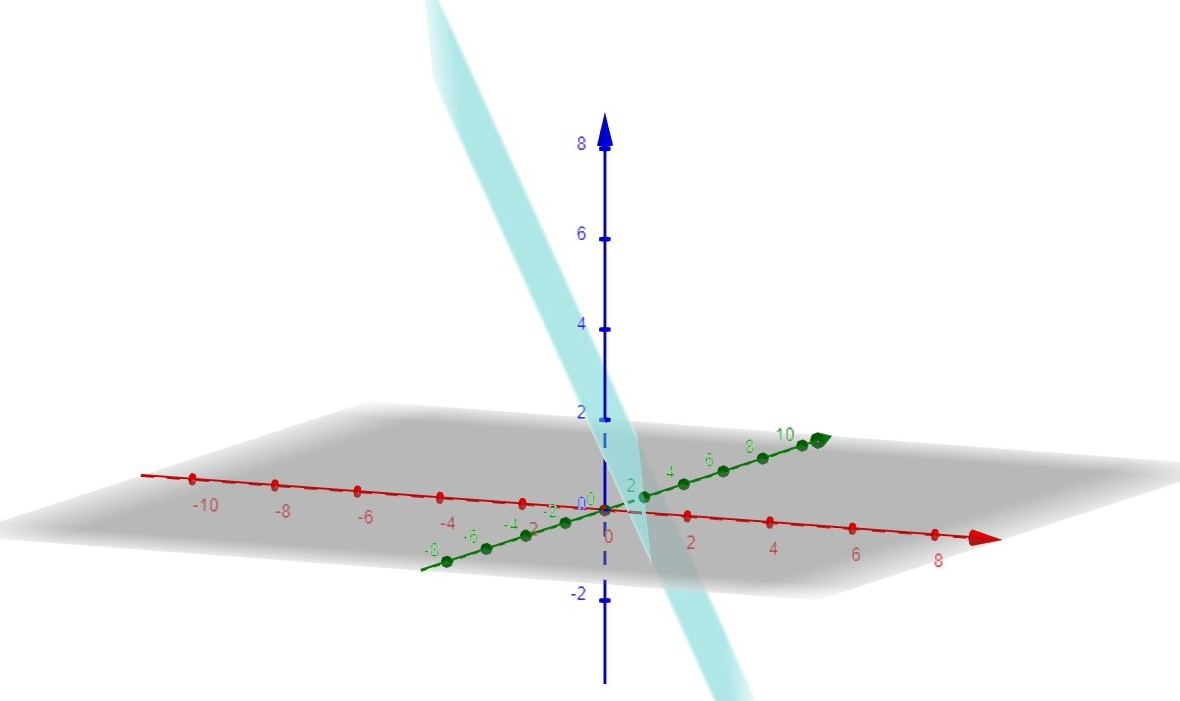
\includegraphics[scale = 0.2]{lec23-2.jpg}\\
	При $z = 0$ вычисляется пересечение $2 -x-y$ с плоскостью $Oxy$ :
	\[\iint \limits_\pi x ds = \iint \limits_D x \sqrt{1 + 4 +1} \  dx dy = 
	\sqrt{6}
	 \int \limits_0^1  dx \int \limits_0^{2 - 2x} x dy = \sqrt 6 \int \limits_0^1 
	 x(2 -2x) \ dx = \frac{\sqrt 6}{3}\] 
	 \end{enumerate}
	\end{exmps}
	\subsection{Свойства ПовИ-1}
	\begin{itemize}
		\item 	Не зависит от выбора стороны поверхности
		\item	В интегральной сумме $\sum\limits_{k} f(x_k, y_k, z_k) \Delta s_k
		 \qquad \Delta s_k = $ площадь $\pi_k$ не связана с выбором стороны 
		 поверхности
		\item Другие свлйства: линейность, аддитивность (обычные для интегралов),
		 основная оценка: если $m \leq f(x, y, z) \leq M, \quad (x, y, z) \in \pi$,
		  то $mS \leq \iint \limits_\pi f(x, y, z) ds \leq MS$, где $S$ \---
		   площадь $\pi$
		\item $\iint \limits_\pi ds  = S = $площадь $\pi$
		\item ПовИ-1 существует для тех функций $f$, для которых существует двойной
		 интеграл в формуле \eqref{lec23-1}. Для этого достаточно, чтобы функция была
		  кусочно-непрерывная и ограниченная.\\
		Вместо гладкой поверхности $\pi$ можно предполагать кусочно-гладкие
		 поверхности, т.~е. такие, которые можно разбить на конечное множество
		  частей, каждая из которых \--- гладкая.\\
		\section{ПовИ-2}
		Пусть задана гладкая двусторонняя квалрируемая поверхность $\pi$. Выберем
		 какую-то сторону поверхности. Так как поверхность гладкая, в каждой точке
		  поверхности есть вектор нормали $\vec{N} = \pm (A, B,C) = \pm
		   [\vec r\,'}_u, \vec{r'_v]$. Выбираем конкретный
		    знак + или -. Тогда во всех точках будет задан $\vec{N}$
		     Единственным образом. Обозначим $\vec{n} =
		      \frac{\vec{N}}{|\vec{N}|}$ \--- имеет
		       единичную длину. Его координатами являются
		       направляющие косинусы
		\[\vec{n} = \frac{\pm(A,B,C)}{\sqrt{A^2 +B^2 + C^2}} = 
		(\cos \alpha, \cos \beta, \cos \gamma).\]
		\subsection{Выбор стороны поверхности}
		Если взять $\pm C$ с таким знаком, что $\pm C > 0$, то тогда $\cos \gamma
		 > 0$ и, значит, $\vec{n}$ и $\vec{N}$ образуют с осью
		  $Oz$ острый угол (можно говорить, что вектор нормали направлен вверх).
		   Это и дает определенную сторону поверхности.\\
		Пусть задана поверхность$\pi$ \--- гдадкая двусторонняя квадрируемая
	 поверхность, на которой определена $R(x,y,z)$. Разобьем $\pi$ на части	
	  $\pi_k$, площадь $\pi_k$ равна $\Delta s_k$. Выберем некоторую сторону
	  поверхности $\pi$ (тогда говорят, что $\pi$ ориентирована). Возьмем
      $M_k(x_k, y_k, z_k) \in \pi_k$. В этой точке есть вектор	
      $\vec{n} =
       (\cos \alpha, \cos \beta, \cos \gamma).$ Обозначим $\Delta \sigma_k = $
        площадь проекции кусочка $\pi_k$ на $Oxy$. Введем в рассмотрение $(\pm
        \Delta\sigma_k),$ где знак \glqq$ + $\grqq, если $\cos \gamma > 0$ и 
        знак
         \glqq$-$ \grqq, если $\cos \gamma < 0$. Построим сумму 
         $\sum\limits_k^n
         R(x_k, y_k, z_k)(\pm \Delta\sigma_k)$. Предел этой суммы обозначают
         $\lim\limits_{\delta \to 0} \sum\limits_k^n R(x_k, y_k, z_k)(\pm
         \Delta\sigma_k) = \iint \limits_\pi R(x, y, z) dx dy $ и называют
         $\emph{поверхностным интегралом второго рода}$ по выьранной стороне
         поверхности $\pi$. Аналогично определяют $\iint \limits_\pi P(x, y, 
         z) 
         dydz,\\ \iint \limits_\pi Q(x, y, z) dxdz $. Обычно рассматривают
          ПовИ-2 общего вида:
		\[\iint \limits_\pi P(x, y, z) dydz + Q(x, y, z) dxdz
		 + R(x, y, z) dxdy \]
		Сразу заметим, что повИ-2 зависит от выбора поверхности (при выборе другой
		 стороны знак поменяется на противоположный).
	\end{itemize}
	\end{document}
